\documentclass[12pt,a4paper]{report}

%Set language
\usepackage[english]{babel}

% To import and adjust images
\usepackage{graphicx}
\usepackage[export]{adjustbox}
\usepackage[center]{caption}
\usepackage{subcaption}

% Path relative to the .tex file containing the \includegraphics command
\graphicspath{ {./images/} }  

% To change the ToC title
\addto\captionsenglish{ \renewcommand {\contentsname} {Table of contents}}

\title{SafeStreets - RASD \\ \large version 1.0}
\author{Frangi Alberto, Fucci Tiziano}
\date{A.Y. 2019/2020}
\begin{document}
\maketitle

% Command to hide subsections in the index
\setcounter{tocdepth}{1}

% Index
\tableofcontents
\chapter{Introduction}
	\section{Purpose}
		\subsection{General Purpose}
SafeStreets is a crowd-sourced application that intends to provide users with the possibility to notify authorities when traffic violations occur, and in particular parking violations, such as vehicles parked in the middle of bike lanes or in places reserved for people with disabilities, double parking, and so on. The application allows users to send pictures of violations, including their date, time, and position, to authorities.
 
SafeStreets stores the information provided by users, completing it with suitable meta-data. In particular, when it receives a picture, it runs an algorithm to read the license plate (one can also think of mechanisms with which the user can help with the recognition), and stores the retrieved information with theviolation, including also the type of the violation (input by the user) and the name of the street where the violation occurred (which can be retrieved from the geographical position of the violation). 

The application allows both end users and authorities to mine the information that has been received, for example by highlighting the streets (or the areas) with the highest frequency of violations, or the vehicles that commit the most violations. 

Moreover, if the municipality offers a service that allows users to retrieve the information about the accidents that occur on the territory of the municipality, SafeStrees can cross this information with its own data to identify potentially unsafe areas, and suggest possible interventions (e.g., add a barrier between the bike lane and the part of the road for motorized vehicles to prevent unsafe parking).

		\subsection{Goals}
The following list describes the goals from the S2B perspective:

% Dot list 
\begin{itemize}
	\item \textbf{G1}: The application must allow users to notify traffic violations, providing date, time, position, the type of violation and a picture of the vehicle.
  	\item \textbf{G2}: The application must allow authorities to retrieve the reports made by all the users at any moment.
	% \item \textbf{G3}: The application must read correctly the license plates from the pictures attached to reports. --assumption?
	\item \textbf{G3}: The application must be able to detect the streets and the vehicles with the highest frequency of violations.
	\item \textbf{G4}: The application must be able to identify potentially unsafe areas and suggest possible interventions.
	\item \textbf{G5}: The application must not show one user's reports to other users.
	\item \textbf{G6}: The application must allow every user to see all of his reports and their status.
\end{itemize}

	\section{Scope}
Safestreet is an application to be used both from civilians (users) and authorities, in order to help the latter and reduce traffic violations. Registered authorities can automatically receive reports made by users, so the service acts as an intermediary. Reports are made of a picture of the violation and some... 
%(to be reviewed and completed)

	\section{Definitions, acronyms, abbreviations}
		\subsection{Definitions}
		\begin{itemize}
		\item \textbf{User}: a civilian customer that can use the application to:
			\begin{itemize}
			\item notify authorities of some violation;
			\item check which are the most dangerous (i.e. with the most violations) streets;
			\item check which are the vehicles that committed the most violations.
			\end{itemize}
		\item \textbf{Authority}: a member of the local police who has access to reports made by users.
		\item \textbf{Report}: a message consisting of:
			\begin{itemize}
			\item a picture showing the car in order to show the occurring violation;
			\item date and time of the picture;
			\item GPS position of the place where the violation occurred;
			\item the street where the violation occurred (automatically retrieved from the geographical position);
			\item the type of the violation (input by the user)
			\end{itemize}
		\item \textbf{Violation}: a situation that, according to the user who sent the report, is a violation of the traffic laws.
		\item \textbf{Intervention}: a brief text suggesting a possible solution in order to improve safety and discourage future violations.
		\end{itemize}
		\subsection{Acronyms}
			\begin{itemize}
			\item \textbf{API}: \emph{Application Programming Interface.}
			\item \textbf{GPS}: \emph{Global Positioning System.}
			\item \textbf{UI}: \emph{User Interface.}		
			\item \textbf{S2B}: \emph{Software-to-be.}	
			\end{itemize}
		\subsection{Abbreviations}
% To be written

	\section{Revision history}
% To be written

	\section{Reference documents}
	\begin{itemize}
	\item {Specification document}: ``SafeStreets Mandatory Project Assignment''
	%to be completed
	\end{itemize}

	\section{Document structure}
	\begin{itemize}
	\item \textbf{Chapter 1} is an introduction: it presents the document and the S2B with its scope and goals. It also helps the reader to understand, by giving the necessary definitions and explaining acronyms and abbreviations. 
	\item \textbf{Chapter 2} is...
	\item \textbf{Chapter 3} is the core of the document...
	\item \textbf{Chapter 4} contains the Alloy model of critical aspects that require special attention. Here it is shown how the project has been modeled and a proof of the model consistency is provided. Moreover, examples of some of the generated world are shown.
	\item \textbf{Chapter 5} is meant to show how work was divided between the two components of the group and how much time was spent.
	\item \textbf{Chapter 6} contains the list of references...
	\end{itemize}

% End of first chapter

\chapter{Overall description}
	\section{Product perspective}
	\section{Product functions}
	\section{User characteristics}
	\section{Assumptions, dependencies and constraints}
% End of second chapter

\chapter{Specific Requirments}
	\section{External interface requirments}
		\subsection{User interfaces}

		\begin{figure}[h]
		\begin{subfigure}{0.5\textwidth}
			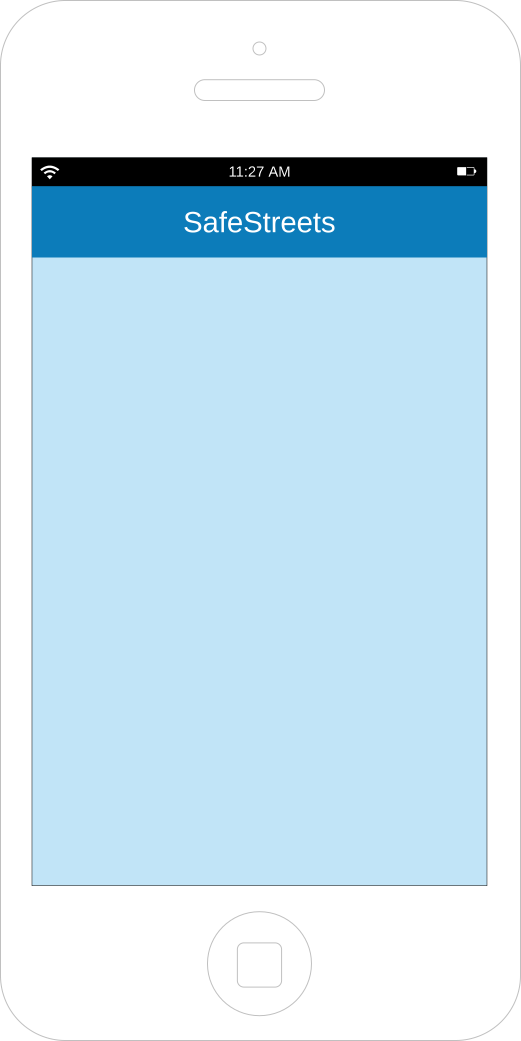
\includegraphics[scale=0.25, center]{Background}
			\caption{Sample text1}
			\label{fig:subim1}
		\end{subfigure}
		\begin{subfigure}{0.5\textwidth}
			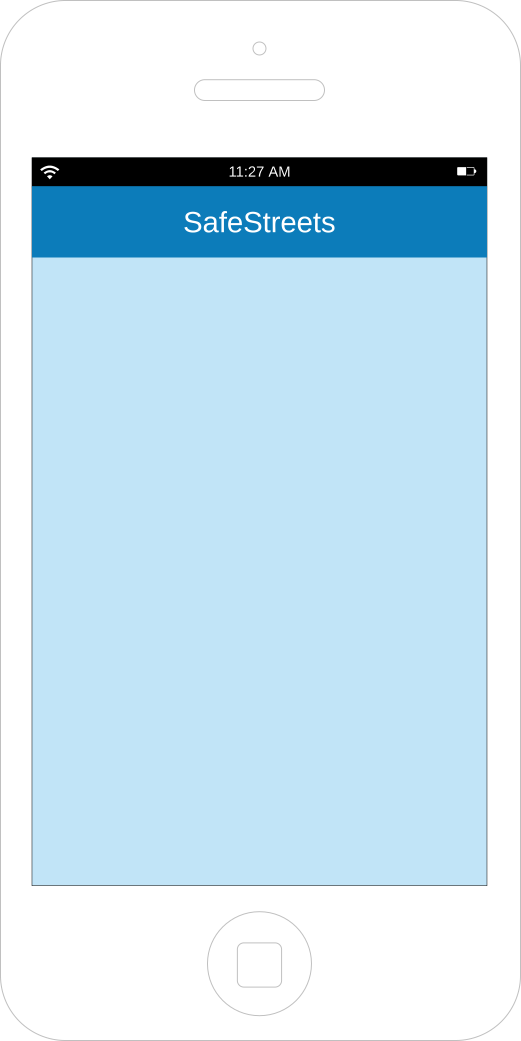
\includegraphics[scale=0.25, center]{Background}
			\caption{Sample text1}
			\label{fig:subim1}
		\end{subfigure}
		\end{figure}

		\begin{figure}
		\begin{subfigure}{0.5\textwidth}
			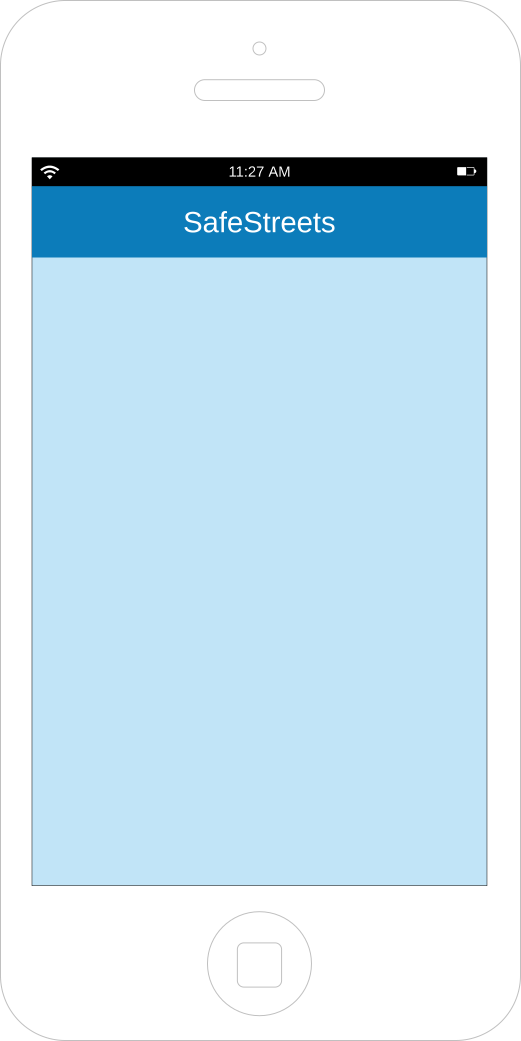
\includegraphics[scale=0.25, center]{Background}
			\caption{Sample text3}
			\label{fig:subim2}
		\end{subfigure}
		\end{figure}

		\subsection{Hardware interfaces}
		\subsection{Software interfaces}
		\subsection{Communication interfaces}
	\section{Functional Requirements}
	\section{Performances Requirments}
	\section{Design constraints}
		\subsection{Standards compliance}
		\subsection{Hardware limitations}
		\subsection{Any other costraint}
	\section{Software System Attributes}
		\subsection{Reliability}
		\subsection{Availability}
		\subsection{Security}
		\subsection{Maintainability}
		\subsection{Portablity}
% End of third chapter

\chapter{Formal Analysis}
% End of fourth chapter

\chapter{Effort Spent}
%End of fifth chapter

\chapter{References}
% End of sixth chapter

\end{document}